\PassOptionsToPackage{unicode=true}{hyperref} % options for packages loaded elsewhere
\PassOptionsToPackage{hyphens}{url}
%
\documentclass[]{article}
\usepackage{lmodern}
\usepackage{amssymb,amsmath}
\usepackage{ifxetex,ifluatex}
\usepackage{fixltx2e} % provides \textsubscript
\ifnum 0\ifxetex 1\fi\ifluatex 1\fi=0 % if pdftex
  \usepackage[T1]{fontenc}
  \usepackage[utf8]{inputenc}
  \usepackage{textcomp} % provides euro and other symbols
\else % if luatex or xelatex
  \usepackage{unicode-math}
  \defaultfontfeatures{Ligatures=TeX,Scale=MatchLowercase}
\fi
% use upquote if available, for straight quotes in verbatim environments
\IfFileExists{upquote.sty}{\usepackage{upquote}}{}
% use microtype if available
\IfFileExists{microtype.sty}{%
\usepackage[]{microtype}
\UseMicrotypeSet[protrusion]{basicmath} % disable protrusion for tt fonts
}{}
\IfFileExists{parskip.sty}{%
\usepackage{parskip}
}{% else
\setlength{\parindent}{0pt}
\setlength{\parskip}{6pt plus 2pt minus 1pt}
}
\usepackage{hyperref}
\hypersetup{
            pdftitle={Bagging and Random Forests},
            pdfauthor={Shan Chen},
            pdfborder={0 0 0},
            breaklinks=true}
\urlstyle{same}  % don't use monospace font for urls
\usepackage[margin=1in]{geometry}
\usepackage{color}
\usepackage{fancyvrb}
\newcommand{\VerbBar}{|}
\newcommand{\VERB}{\Verb[commandchars=\\\{\}]}
\DefineVerbatimEnvironment{Highlighting}{Verbatim}{commandchars=\\\{\}}
% Add ',fontsize=\small' for more characters per line
\usepackage{framed}
\definecolor{shadecolor}{RGB}{248,248,248}
\newenvironment{Shaded}{\begin{snugshade}}{\end{snugshade}}
\newcommand{\AlertTok}[1]{\textcolor[rgb]{0.94,0.16,0.16}{#1}}
\newcommand{\AnnotationTok}[1]{\textcolor[rgb]{0.56,0.35,0.01}{\textbf{\textit{#1}}}}
\newcommand{\AttributeTok}[1]{\textcolor[rgb]{0.77,0.63,0.00}{#1}}
\newcommand{\BaseNTok}[1]{\textcolor[rgb]{0.00,0.00,0.81}{#1}}
\newcommand{\BuiltInTok}[1]{#1}
\newcommand{\CharTok}[1]{\textcolor[rgb]{0.31,0.60,0.02}{#1}}
\newcommand{\CommentTok}[1]{\textcolor[rgb]{0.56,0.35,0.01}{\textit{#1}}}
\newcommand{\CommentVarTok}[1]{\textcolor[rgb]{0.56,0.35,0.01}{\textbf{\textit{#1}}}}
\newcommand{\ConstantTok}[1]{\textcolor[rgb]{0.00,0.00,0.00}{#1}}
\newcommand{\ControlFlowTok}[1]{\textcolor[rgb]{0.13,0.29,0.53}{\textbf{#1}}}
\newcommand{\DataTypeTok}[1]{\textcolor[rgb]{0.13,0.29,0.53}{#1}}
\newcommand{\DecValTok}[1]{\textcolor[rgb]{0.00,0.00,0.81}{#1}}
\newcommand{\DocumentationTok}[1]{\textcolor[rgb]{0.56,0.35,0.01}{\textbf{\textit{#1}}}}
\newcommand{\ErrorTok}[1]{\textcolor[rgb]{0.64,0.00,0.00}{\textbf{#1}}}
\newcommand{\ExtensionTok}[1]{#1}
\newcommand{\FloatTok}[1]{\textcolor[rgb]{0.00,0.00,0.81}{#1}}
\newcommand{\FunctionTok}[1]{\textcolor[rgb]{0.00,0.00,0.00}{#1}}
\newcommand{\ImportTok}[1]{#1}
\newcommand{\InformationTok}[1]{\textcolor[rgb]{0.56,0.35,0.01}{\textbf{\textit{#1}}}}
\newcommand{\KeywordTok}[1]{\textcolor[rgb]{0.13,0.29,0.53}{\textbf{#1}}}
\newcommand{\NormalTok}[1]{#1}
\newcommand{\OperatorTok}[1]{\textcolor[rgb]{0.81,0.36,0.00}{\textbf{#1}}}
\newcommand{\OtherTok}[1]{\textcolor[rgb]{0.56,0.35,0.01}{#1}}
\newcommand{\PreprocessorTok}[1]{\textcolor[rgb]{0.56,0.35,0.01}{\textit{#1}}}
\newcommand{\RegionMarkerTok}[1]{#1}
\newcommand{\SpecialCharTok}[1]{\textcolor[rgb]{0.00,0.00,0.00}{#1}}
\newcommand{\SpecialStringTok}[1]{\textcolor[rgb]{0.31,0.60,0.02}{#1}}
\newcommand{\StringTok}[1]{\textcolor[rgb]{0.31,0.60,0.02}{#1}}
\newcommand{\VariableTok}[1]{\textcolor[rgb]{0.00,0.00,0.00}{#1}}
\newcommand{\VerbatimStringTok}[1]{\textcolor[rgb]{0.31,0.60,0.02}{#1}}
\newcommand{\WarningTok}[1]{\textcolor[rgb]{0.56,0.35,0.01}{\textbf{\textit{#1}}}}
\usepackage{graphicx,grffile}
\makeatletter
\def\maxwidth{\ifdim\Gin@nat@width>\linewidth\linewidth\else\Gin@nat@width\fi}
\def\maxheight{\ifdim\Gin@nat@height>\textheight\textheight\else\Gin@nat@height\fi}
\makeatother
% Scale images if necessary, so that they will not overflow the page
% margins by default, and it is still possible to overwrite the defaults
% using explicit options in \includegraphics[width, height, ...]{}
\setkeys{Gin}{width=\maxwidth,height=\maxheight,keepaspectratio}
\setlength{\emergencystretch}{3em}  % prevent overfull lines
\providecommand{\tightlist}{%
  \setlength{\itemsep}{0pt}\setlength{\parskip}{0pt}}
\setcounter{secnumdepth}{0}
% Redefines (sub)paragraphs to behave more like sections
\ifx\paragraph\undefined\else
\let\oldparagraph\paragraph
\renewcommand{\paragraph}[1]{\oldparagraph{#1}\mbox{}}
\fi
\ifx\subparagraph\undefined\else
\let\oldsubparagraph\subparagraph
\renewcommand{\subparagraph}[1]{\oldsubparagraph{#1}\mbox{}}
\fi

% set default figure placement to htbp
\makeatletter
\def\fps@figure{htbp}
\makeatother


\title{Bagging and Random Forests}
\author{Shan Chen}
\date{4/20/2020}

\begin{document}
\maketitle

\hypertarget{setup}{%
\section{Setup}\label{setup}}

Load in some synthetic data so use with Decision Trees.

\begin{Shaded}
\begin{Highlighting}[]
\NormalTok{dataDir <-}\StringTok{ "/Users/shawnchen/Desktop/rzhw"}
\NormalTok{file1 <-}\StringTok{ "RectData_Quant.csv"}
\NormalTok{file2 <-}\StringTok{ "Classify2D_Data3.csv"}
\NormalTok{regData.df <-}\StringTok{ }\KeywordTok{read.csv}\NormalTok{(}\KeywordTok{file.path}\NormalTok{(dataDir,file1))}
\NormalTok{classData.df <-}\StringTok{ }\KeywordTok{read.csv}\NormalTok{(}\KeywordTok{file.path}\NormalTok{(dataDir,file2)) }\OperatorTok\StringTok{ }
\StringTok{  }\KeywordTok{select}\NormalTok{(}\OperatorTok{-}\NormalTok{row)}
\end{Highlighting}
\end{Shaded}

And the libraries\ldots{}.

\begin{Shaded}
\begin{Highlighting}[]
\KeywordTok{library}\NormalTok{(tidyverse)}
\KeywordTok{library}\NormalTok{(tree)}
\end{Highlighting}
\end{Shaded}

\begin{verbatim}
## Registered S3 method overwritten by 'tree':
##   method     from
##   print.tree cli
\end{verbatim}

\begin{Shaded}
\begin{Highlighting}[]
\NormalTok{data.df <-}\StringTok{ }\NormalTok{classData.df }

\NormalTok{doBootPlot <-}\StringTok{ }\ControlFlowTok{function}\NormalTok{(minDev,minSize)\{}
\NormalTok{  N <-}\StringTok{ }\KeywordTok{nrow}\NormalTok{(data.df)}
\NormalTok{  boots <-}\StringTok{ }\KeywordTok{sample}\NormalTok{(}\DecValTok{1}\OperatorTok{:}\NormalTok{N,N,}\DataTypeTok{rep=}\NormalTok{T)}
\NormalTok{  boot.df <-}\StringTok{ }\NormalTok{data.df[boots,]}
\NormalTok{  mod.tree <-}\StringTok{ }\KeywordTok{tree}\NormalTok{(class }\OperatorTok{~}\StringTok{ }\NormalTok{x }\OperatorTok{+}\StringTok{ }\NormalTok{y, }
                   \DataTypeTok{data=}\NormalTok{boot.df,}
                   \DataTypeTok{control=}\KeywordTok{tree.control}\NormalTok{(}\KeywordTok{nrow}\NormalTok{(boot.df),}
                                        \DataTypeTok{mindev=}\NormalTok{minDev,}
                                        \DataTypeTok{minsize=}\NormalTok{minSize))  }
  \KeywordTok{plot}\NormalTok{(mod.tree)}
\NormalTok{\}}
\end{Highlighting}
\end{Shaded}

These are very different. This is a major deficit of decision trees.
Small changes in the data result in large changes in the resulting tree.
This effect gets more pronounced as the trees get deeper.

\begin{Shaded}
\begin{Highlighting}[]
\KeywordTok{doBootPlot}\NormalTok{(.}\DecValTok{0001}\NormalTok{,}\DecValTok{10}\NormalTok{)}
\end{Highlighting}
\end{Shaded}

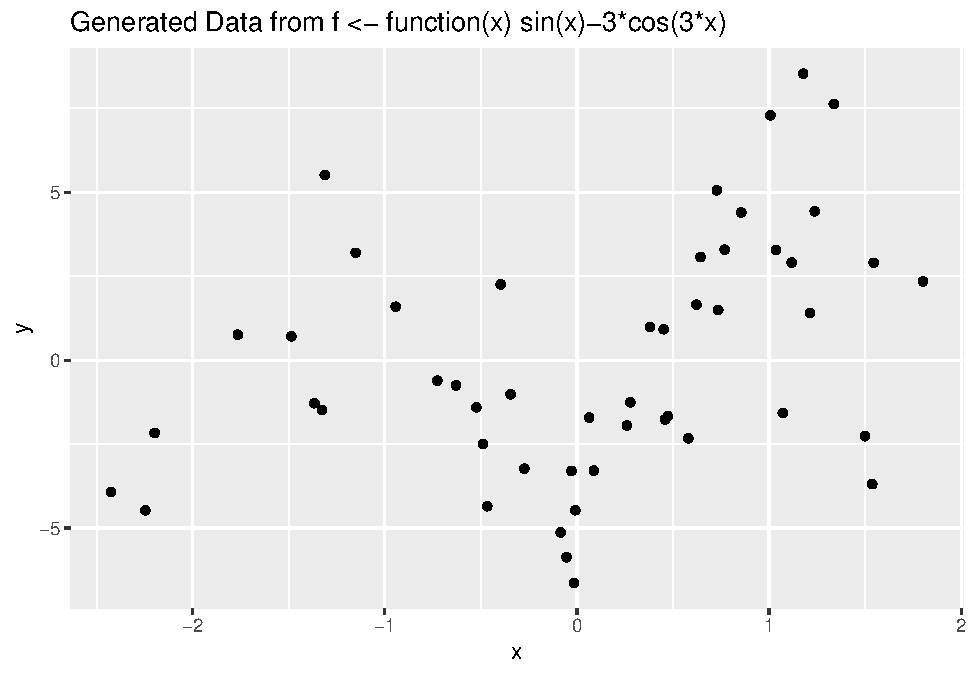
\includegraphics{introbagging_files/figure-latex/unnamed-chunk-4-1.pdf}

\begin{Shaded}
\begin{Highlighting}[]
\KeywordTok{doBootPlot}\NormalTok{(.}\DecValTok{0001}\NormalTok{,}\DecValTok{10}\NormalTok{)}
\end{Highlighting}
\end{Shaded}

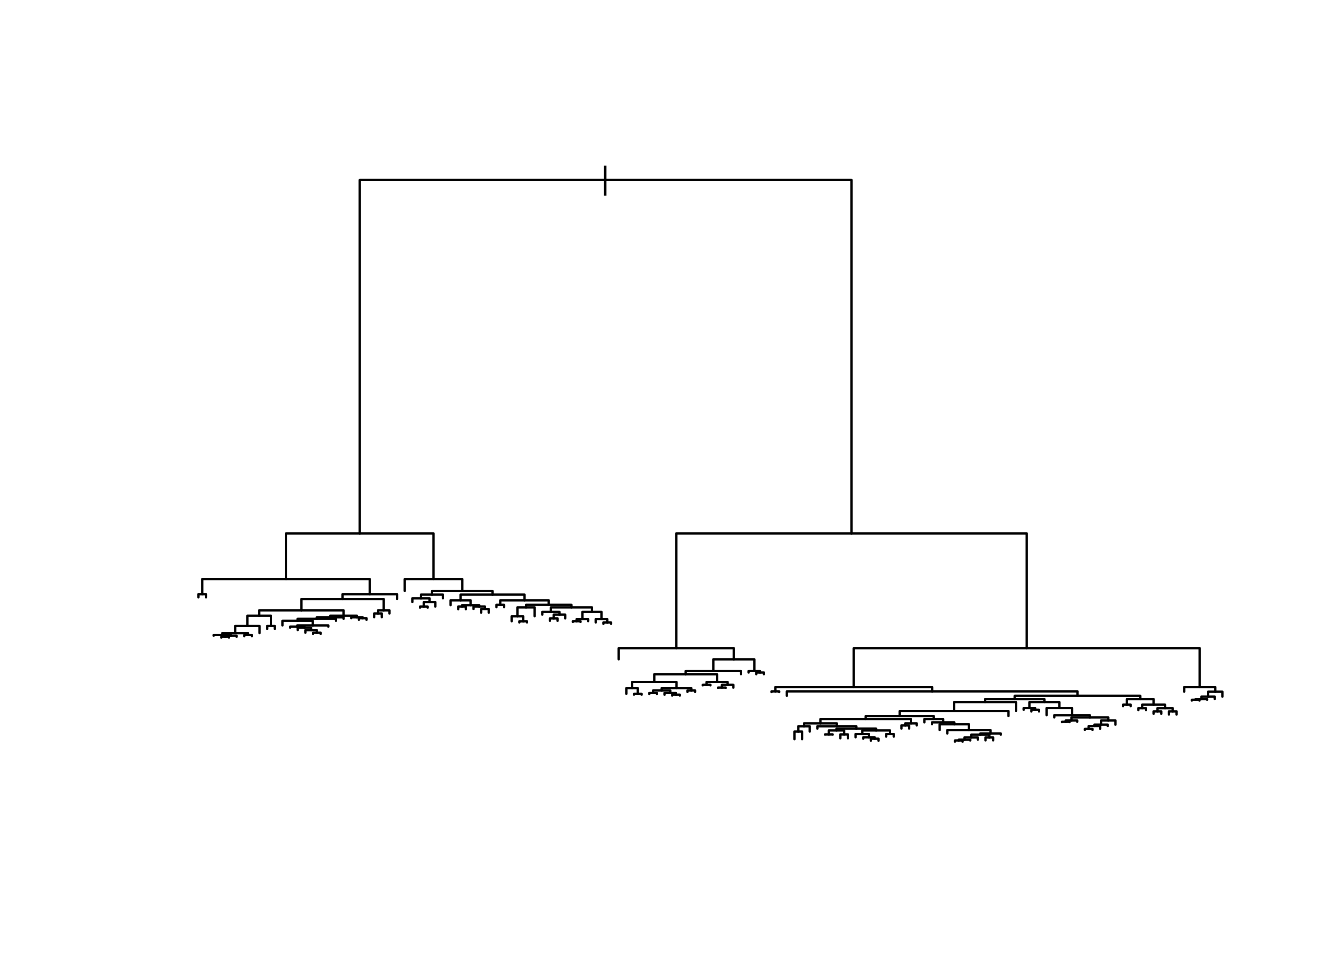
\includegraphics{introbagging_files/figure-latex/unnamed-chunk-4-2.pdf}

\begin{Shaded}
\begin{Highlighting}[]
\KeywordTok{doBootPlot}\NormalTok{(.}\DecValTok{0001}\NormalTok{,}\DecValTok{10}\NormalTok{)}
\end{Highlighting}
\end{Shaded}

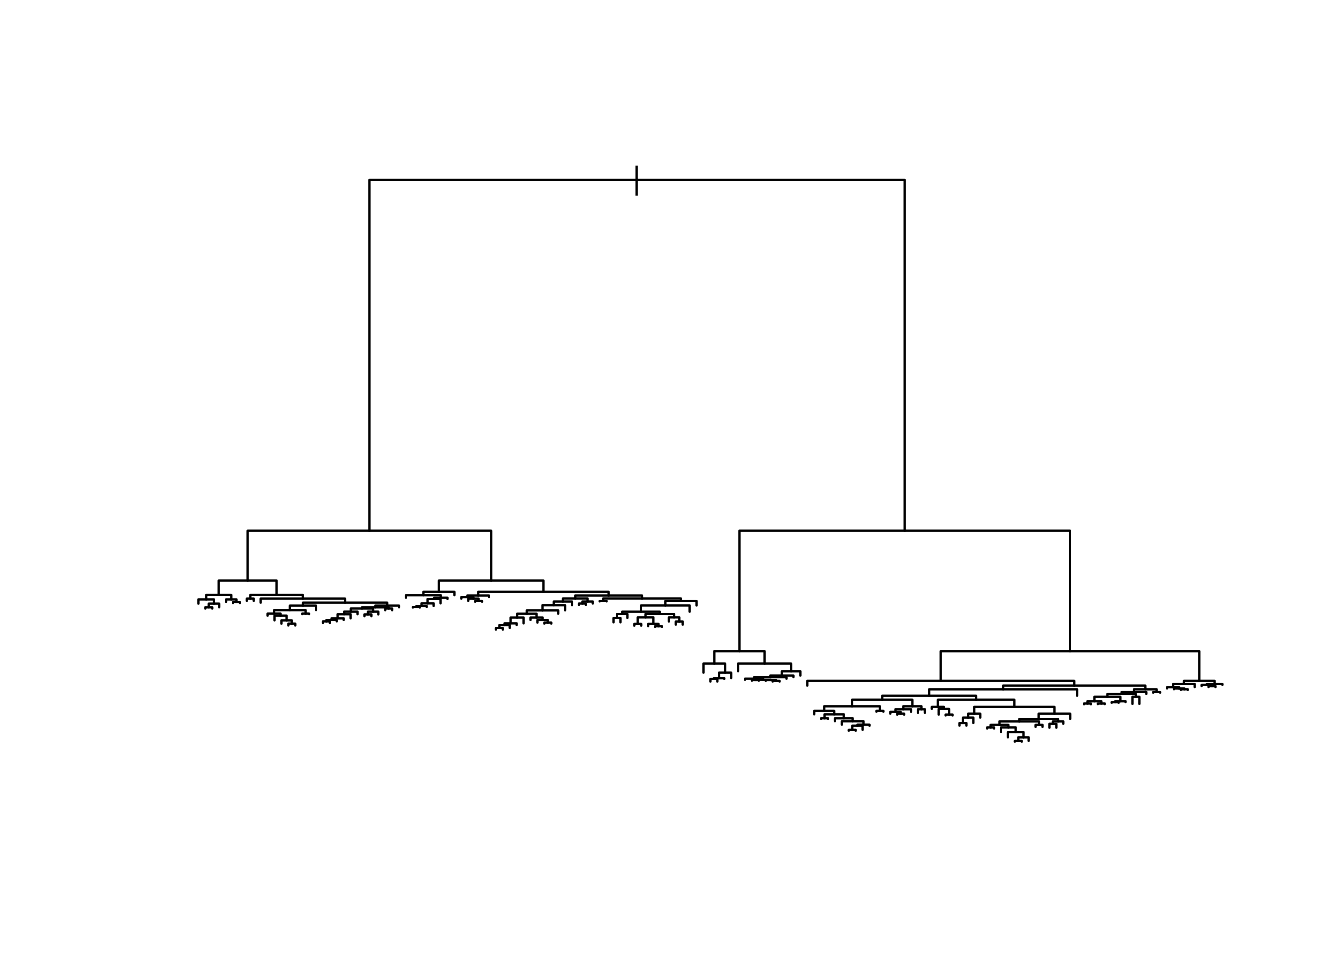
\includegraphics{introbagging_files/figure-latex/unnamed-chunk-4-3.pdf}

\begin{Shaded}
\begin{Highlighting}[]
\KeywordTok{doBootPlot}\NormalTok{(.}\DecValTok{0001}\NormalTok{,}\DecValTok{10}\NormalTok{)}
\end{Highlighting}
\end{Shaded}

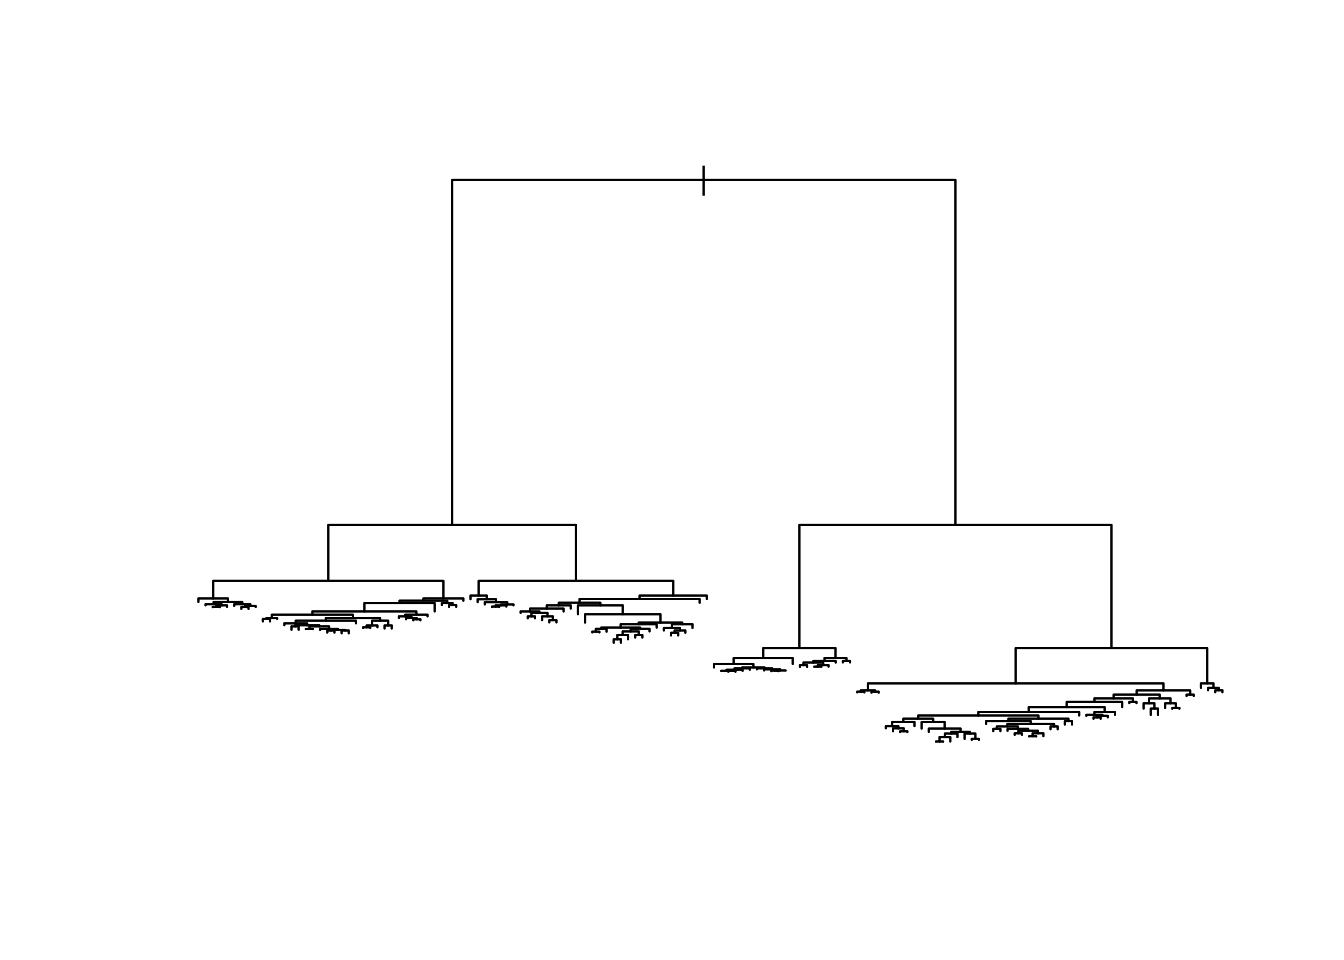
\includegraphics{introbagging_files/figure-latex/unnamed-chunk-4-4.pdf}

\hypertarget{bagging-basics}{%
\section{Bagging Basics}\label{bagging-basics}}

We can turn this deficit into an advantage. Here's the idea. For a given
data set, generate a large number of bootstrapped data sets. For each
build a \textbf{deep} regression tree. To make a prediction on new
value, run the new value through \textbf{all} of the trees. Use the mean
(or majority, if classification) as your prediction.

This is called Bagging, for Bootstrap Aggregation.

Let's do it by hand on our data. Notice that after building our
bootstrapped data set, there will be a bunch of observations left over.
These are called ``Out of Bag'' (OOB). We can use these to compute an
estimate test error! That is, we do some cross-validation on the fly.

\begin{Shaded}
\begin{Highlighting}[]
\NormalTok{N <-}\StringTok{ }\KeywordTok{nrow}\NormalTok{(classData.df)}

\NormalTok{n <-}\StringTok{ }\DecValTok{200}
\NormalTok{build <-}\StringTok{ }\KeywordTok{sample}\NormalTok{(}\DecValTok{1}\OperatorTok{:}\NormalTok{N,n,}\DataTypeTok{rep=}\NormalTok{F)}
\NormalTok{data.df <-}\StringTok{ }\NormalTok{classData.df[build,]}

\CommentTok{##Use this later}
\NormalTok{test <-}\StringTok{ }\KeywordTok{sample}\NormalTok{(}\KeywordTok{setdiff}\NormalTok{(}\DecValTok{1}\OperatorTok{:}\NormalTok{N,build),n,}\DataTypeTok{rep=}\NormalTok{F)}
\NormalTok{test.df <-}\StringTok{ }\NormalTok{classData.df[test,]}
\end{Highlighting}
\end{Shaded}

Let's build a bagged set of trees.

\begin{Shaded}
\begin{Highlighting}[]
\KeywordTok{dim}\NormalTok{(data.df)}
\end{Highlighting}
\end{Shaded}

\begin{verbatim}
## [1] 200   3
\end{verbatim}

\begin{Shaded}
\begin{Highlighting}[]
\NormalTok{numBoots <-}\StringTok{ }\DecValTok{100}
\NormalTok{minDev <-}\StringTok{ }\FloatTok{.0001}
\NormalTok{minSize <-}\StringTok{ }\DecValTok{4}
\NormalTok{numPred <-}\StringTok{ }\KeywordTok{ncol}\NormalTok{(data.df)}\OperatorTok{-}\DecValTok{1}
\CommentTok{## Here's where we keep our trees and the errors}
\CommentTok{## Note: this has to be a list to handle complex objecsts}
\CommentTok{## such as trees.}
\NormalTok{bootedTrees <-}\StringTok{ }\KeywordTok{list}\NormalTok{()}
\NormalTok{oobErrs <-}\StringTok{ }\KeywordTok{numeric}\NormalTok{(numBoots)}

\ControlFlowTok{for}\NormalTok{(k }\ControlFlowTok{in} \DecValTok{1}\OperatorTok{:}\NormalTok{numBoots)\{}
\NormalTok{  boots <-}\StringTok{ }\KeywordTok{sample}\NormalTok{(}\DecValTok{1}\OperatorTok{:}\NormalTok{n,n,}\DataTypeTok{rep=}\NormalTok{T)}
\NormalTok{  boot.df <-}\StringTok{ }\NormalTok{data.df[boots,]}
  \CommentTok{## Left over observations =  Out Of Bags (OOBs) }
\NormalTok{  oobs <-}\StringTok{ }\KeywordTok{setdiff}\NormalTok{(}\DecValTok{1}\OperatorTok{:}\NormalTok{n,boots)}
\NormalTok{  oob.df <-}\StringTok{ }\NormalTok{data.df[oobs,]}
  \CommentTok{#### Build the tree}
\NormalTok{  bootedTree<-}\StringTok{ }\KeywordTok{tree}\NormalTok{(class }\OperatorTok{~}\StringTok{ }\NormalTok{x }\OperatorTok{+}\StringTok{ }\NormalTok{y, }
                    \DataTypeTok{data=}\NormalTok{boot.df,}
                    \DataTypeTok{control=}\KeywordTok{tree.control}\NormalTok{(}\KeywordTok{nrow}\NormalTok{(boot.df),}
                                         \DataTypeTok{mindev=}\FloatTok{0.0001}\NormalTok{,}
                                         \DataTypeTok{minsize=}\DecValTok{4}\NormalTok{))}
  \CommentTok{## Predict on the OOBs}
\NormalTok{  preds <-}\StringTok{ }\KeywordTok{predict}\NormalTok{(bootedTree,}
                   \DataTypeTok{newdata=}\NormalTok{oob.df,}
                   \DataTypeTok{type=}\StringTok{"class"}\NormalTok{)}
  \CommentTok{##compute the error rate}
\NormalTok{  oobErrs[k] <-}\StringTok{ }\KeywordTok{with}\NormalTok{(oob.df,}\KeywordTok{mean}\NormalTok{(class }\OperatorTok{!=}\StringTok{ }\NormalTok{preds))}
  \CommentTok{##keep the trees.. these are the predictive model}
\NormalTok{  bootedTrees[[k]] <-}\StringTok{ }\NormalTok{bootedTree}
\NormalTok{\}}
\end{Highlighting}
\end{Shaded}

From the obbErrs we can get a rough estimate of the error rate. Turns
out we, can do slightly better. More on this later

\begin{Shaded}
\begin{Highlighting}[]
\CommentTok{##estimate the error}
\KeywordTok{mean}\NormalTok{(oobErrs)}
\end{Highlighting}
\end{Shaded}

\begin{verbatim}
## [1] 0.2100376
\end{verbatim}

Not too bad. We now want to use all these bootstrapped trees to make
predictions on any data frame.

The function that does this is pretty straight forward. For an arbitrary
data frame, run through the list of booted trees and make the
predictions. Store the results and use that to make a prediction based
on majority vote.

\begin{Shaded}
\begin{Highlighting}[]
\CommentTok{## T}
\NormalTok{probBoot <-}\StringTok{ }\ControlFlowTok{function}\NormalTok{(data.df,bootTrees)\{}
\NormalTok{  numBoots <-}\StringTok{ }\KeywordTok{length}\NormalTok{(bootTrees)}
  \CommentTok{##row for each observation, column for each boot}
\NormalTok{  preds <-}\StringTok{ }\KeywordTok{matrix}\NormalTok{(}\DataTypeTok{nrow=}\KeywordTok{nrow}\NormalTok{(data.df),}
                  \DataTypeTok{ncol=}\NormalTok{numBoots)}
  \ControlFlowTok{for}\NormalTok{(k }\ControlFlowTok{in} \DecValTok{1}\OperatorTok{:}\NormalTok{numBoots)\{}
\NormalTok{    preds[,k]  <-}\StringTok{ }\KeywordTok{predict}\NormalTok{(bootTrees[[k]],}\DataTypeTok{newdata=}\NormalTok{data.df,}\DataTypeTok{type=}\StringTok{"class"}\NormalTok{)}
\NormalTok{  \}}
  \CommentTok{##take a vote across the rows to get a prediction}
  \CommentTok{## For each observation, returns the proportion of predictions}
  \CommentTok{## that are in the  first class.}
  \KeywordTok{apply}\NormalTok{(preds}\OperatorTok{==}\StringTok{"1"}\NormalTok{,}\DecValTok{1}\NormalTok{,mean)}
\NormalTok{\}}
\end{Highlighting}
\end{Shaded}

\begin{Shaded}
\begin{Highlighting}[]
\NormalTok{probs <-}\StringTok{ }\KeywordTok{probBoot}\NormalTok{(test.df,bootedTrees)}
\KeywordTok{with}\NormalTok{(test.df,}\KeywordTok{table}\NormalTok{(class,probs }\OperatorTok{<}\StringTok{ }\FloatTok{0.5}\NormalTok{))}
\end{Highlighting}
\end{Shaded}

\begin{verbatim}
##      
## class FALSE TRUE
##     A   102   14
##     B    19   65
\end{verbatim}

\begin{Shaded}
\begin{Highlighting}[]
\NormalTok{(err.bag <-}\StringTok{ }\KeywordTok{with}\NormalTok{(test.df,}\KeywordTok{mean}\NormalTok{((class}\OperatorTok{==}\StringTok{"B"}\NormalTok{) }\OperatorTok{!=}\StringTok{ }\NormalTok{(probs }\OperatorTok{<}\StringTok{ }\FloatTok{0.5}\NormalTok{))))}
\end{Highlighting}
\end{Shaded}

\begin{verbatim}
## [1] 0.165
\end{verbatim}

\hypertarget{comparison-with-logistic-regression}{%
\subsection{Comparison with Logistic
Regression}\label{comparison-with-logistic-regression}}

Compare with logistic regression\ldots{}

\begin{Shaded}
\begin{Highlighting}[]
\NormalTok{mod.log <-}\StringTok{ }\KeywordTok{glm}\NormalTok{(class }\OperatorTok{~}\StringTok{ }\NormalTok{x }\OperatorTok{+}\StringTok{ }\NormalTok{y,}
               \DataTypeTok{data=}\NormalTok{data.df,}
               \DataTypeTok{family=}\StringTok{"binomial"}\NormalTok{)}
\NormalTok{probs.log <-}\StringTok{ }\KeywordTok{predict}\NormalTok{(mod.log,}
                     \DataTypeTok{newdata=}\NormalTok{test.df,}
                     \DataTypeTok{type=}\StringTok{"response"}\NormalTok{)}
\KeywordTok{with}\NormalTok{(test.df,}\KeywordTok{table}\NormalTok{(class,probs.log }\OperatorTok{>}\StringTok{ }\FloatTok{0.5}\NormalTok{))}
\end{Highlighting}
\end{Shaded}

\begin{verbatim}
##      
## class FALSE TRUE
##     A   105   11
##     B    17   67
\end{verbatim}

\begin{Shaded}
\begin{Highlighting}[]
\NormalTok{(err.log <-}\StringTok{ }\KeywordTok{with}\NormalTok{(test.df,}\KeywordTok{mean}\NormalTok{((class}\OperatorTok{==}\StringTok{"B"}\NormalTok{) }\OperatorTok{!=}\StringTok{ }\NormalTok{(probs.log }\OperatorTok{>}\StringTok{ }\FloatTok{0.5}\NormalTok{))))}
\end{Highlighting}
\end{Shaded}

\begin{verbatim}
## [1] 0.14
\end{verbatim}

\begin{Shaded}
\begin{Highlighting}[]
\KeywordTok{c}\NormalTok{(err.bag,err.log)}
\end{Highlighting}
\end{Shaded}

\begin{verbatim}
## [1] 0.165 0.140
\end{verbatim}

In this case, it looks as if this simple ``bagging'' of trees works at
least as well, if not better than, logistic regression. Of course, YMMV,
but it turns out that bagging is a a very effective modeling tool. It
works especially well in situations where there a large number of
predictors.

\hypertarget{bagging-in-r}{%
\section{Bagging in R}\label{bagging-in-r}}

Of course, R has very efficients functions for doing bagging.

The bagging function is a special case of what is called a Random Forest
(of trees).

\begin{Shaded}
\begin{Highlighting}[]
\KeywordTok{library}\NormalTok{(randomForest)}
\end{Highlighting}
\end{Shaded}

\begin{verbatim}
## randomForest 4.6-14
\end{verbatim}

\begin{verbatim}
## Type rfNews() to see new features/changes/bug fixes.
\end{verbatim}

\begin{verbatim}
## 
## Attaching package: 'randomForest'
\end{verbatim}

\begin{verbatim}
## The following object is masked from 'package:dplyr':
## 
##     combine
\end{verbatim}

\begin{verbatim}
## The following object is masked from 'package:ggplot2':
## 
##     margin
\end{verbatim}

\hypertarget{bagged-classification-trees-in-r}{%
\subsection{Bagged Classification Trees in
R}\label{bagged-classification-trees-in-r}}

We can recreate the bagging from above using randomForest.

\begin{Shaded}
\begin{Highlighting}[]
\NormalTok{numTree <-}\StringTok{ }\DecValTok{100}
\NormalTok{numPred <-}\StringTok{ }\DecValTok{2}
\NormalTok{mod.bag <-}\StringTok{ }\KeywordTok{randomForest}\NormalTok{(class }\OperatorTok{~}\StringTok{ }\NormalTok{x }\OperatorTok{+}\StringTok{ }\NormalTok{y,}
                        \DataTypeTok{data=}\NormalTok{data.df,}
                        \DataTypeTok{ntree=}\NormalTok{numTree,}
                        \DataTypeTok{mtry=}\NormalTok{numPred) }\CommentTok{##mtry=2 = Number of predictors}
\NormalTok{mod.bag}
\end{Highlighting}
\end{Shaded}

\begin{verbatim}
## 
## Call:
##  randomForest(formula = class ~ x + y, data = data.df, ntree = numTree,      mtry = numPred) 
##                Type of random forest: classification
##                      Number of trees: 100
## No. of variables tried at each split: 2
## 
##         OOB estimate of  error rate: 20%
## Confusion matrix:
##    A  B class.error
## A 97 20   0.1709402
## B 20 63   0.2409639
\end{verbatim}

The randomForest function use the OOB values to compute a prediction for
each observation. The idea is simple. As it goes through the boots, it
keeps track of the OOB predictions. Of course, only a fraction of the
observations are present in any one OOB. But over the course of the
bootstrapping, each observation gets predicted a fair number of times
(about numTrees/3, as it turns out). The majority vote of each of these
is the prediction. From this the OOB estimate of the error rate is
determined.

\hypertarget{assignment}{%
\subsection{Assignment}\label{assignment}}

Modify our bootstrapped method above so that it computes a class
prediction for each observation. Make sure that your results agree (up
to randomness) with the randomForest function.

Plan: Create a matrix with one row for each observation and one column
for each tree (bootstrap). Each time through, put the OOB predictions
into their rows of the matrix (the column is the current boot strap
index). Careful: the predictions from the tree are usually given values
1,2, instead of ``A'', ``B''.

When done, do a majority vote across each row. In each row, only about
1/3 of the values will be filled in. You have to ignore the NAs.

\begin{verbatim}
##      preds
## class  A  B
##     A 98 19
##     B 20 63
\end{verbatim}

\begin{verbatim}
## [1] 0.195
\end{verbatim}

\begin{verbatim}
##      oobPred
## class  A  B
##     A 98 19
##     B 20 63
\end{verbatim}

\begin{verbatim}
## [1] 0.195
\end{verbatim}

There is a built-in plot function showing the error rate as the number
of trees increases.

\begin{Shaded}
\begin{Highlighting}[]
\KeywordTok{plot}\NormalTok{(mod.bag)}
\end{Highlighting}
\end{Shaded}

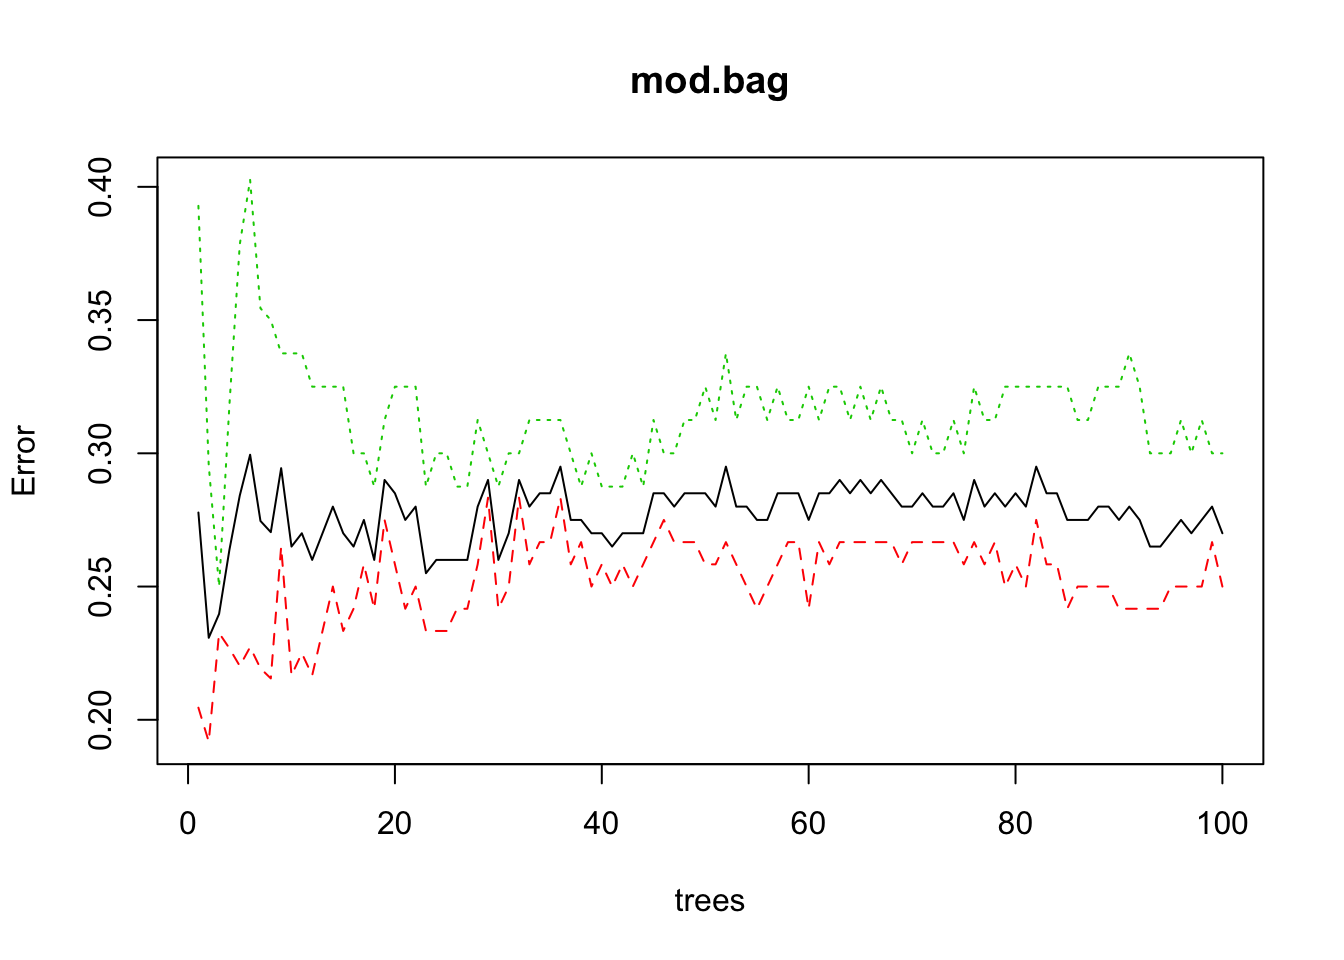
\includegraphics{introbagging_files/figure-latex/unnamed-chunk-12-1.pdf}

As usual, predictions are straightforward.

\begin{Shaded}
\begin{Highlighting}[]
\NormalTok{preds <-}\StringTok{ }\KeywordTok{predict}\NormalTok{(mod.bag,}\DataTypeTok{newdata=}\NormalTok{test.df)}
\KeywordTok{with}\NormalTok{(test.df,}\KeywordTok{table}\NormalTok{(class,preds))}
\end{Highlighting}
\end{Shaded}

\begin{verbatim}
##      preds
## class   A   B
##     A 104  12
##     B  17  67
\end{verbatim}

\begin{Shaded}
\begin{Highlighting}[]
\KeywordTok{with}\NormalTok{(test.df,}\KeywordTok{mean}\NormalTok{(class }\OperatorTok{!=}\StringTok{ }\NormalTok{preds))}
\end{Highlighting}
\end{Shaded}

\begin{verbatim}
## [1] 0.145
\end{verbatim}

Again, about the same error rate.

\hypertarget{solubility-data-set}{%
\section{Solubility Data Set}\label{solubility-data-set}}

Now we look at a real data set. The data are trying to related various
chemical properties to solubility. The response variable, solubility, is
continuous.

Hence we are doing Regression, not Classification, trees. For the most
part, things work about the same way.

Get a look at the data.

\begin{Shaded}
\begin{Highlighting}[]
\NormalTok{solubil.df <-}\StringTok{ }\KeywordTok{read.csv}\NormalTok{(}\StringTok{"APM_Solubility.csv"}\NormalTok{)}
\KeywordTok{dim}\NormalTok{(solubil.df)}
\end{Highlighting}
\end{Shaded}

\begin{verbatim}
## [1] 1267  229
\end{verbatim}

\begin{Shaded}
\begin{Highlighting}[]
\KeywordTok{head}\NormalTok{(}\KeywordTok{names}\NormalTok{(solubil.df))}
\end{Highlighting}
\end{Shaded}

\begin{verbatim}
## [1] "FP001" "FP002" "FP003" "FP004" "FP005" "FP006"
\end{verbatim}

\begin{Shaded}
\begin{Highlighting}[]
\NormalTok{N <-}\StringTok{ }\KeywordTok{nrow}\NormalTok{(solubil.df)}
\NormalTok{numPred <-}\StringTok{ }\KeywordTok{ncol}\NormalTok{(solubil.df)}\OperatorTok{-}\DecValTok{1}
\end{Highlighting}
\end{Shaded}

You could do a correlation plot here to get a feel for the relationship
between the predictors.

\hypertarget{testvalidation-data.}{%
\subsection{Test/validation data.}\label{testvalidation-data.}}

Extract a data set on which to build the model and another data set on
which to test/validate the results.

\begin{Shaded}
\begin{Highlighting}[]
\NormalTok{n <-}\StringTok{ }\DecValTok{500}
\NormalTok{build <-}\StringTok{ }\KeywordTok{sample}\NormalTok{(}\DecValTok{1}\OperatorTok{:}\NormalTok{N,n,}\DataTypeTok{rep=}\NormalTok{F)}
\NormalTok{data.df <-}\StringTok{ }\NormalTok{solubil.df[build,]}

\CommentTok{##Data to test/validate the model}
\NormalTok{n <-}\StringTok{ }\DecValTok{500}
\NormalTok{test <-}\StringTok{ }\KeywordTok{sample}\NormalTok{(}\KeywordTok{setdiff}\NormalTok{(}\DecValTok{1}\OperatorTok{:}\NormalTok{N,build),n,}\DataTypeTok{rep=}\NormalTok{F)}
\NormalTok{test.df <-}\StringTok{ }\NormalTok{solubil.df[test,]}
\end{Highlighting}
\end{Shaded}

Now we can buld a build a Bagged model with 100 tees using the R
randomForest function.

Again, in randomForest that is a argument (mtry) which indicates the
number of predictors to use at each branch. For now, we'll use all the
predictors. Later, we'll limit the number of predictors.

\begin{Shaded}
\begin{Highlighting}[]
\NormalTok{numTree <-}\StringTok{ }\DecValTok{100}
\NormalTok{mod.bag <-}\StringTok{ }\KeywordTok{randomForest}\NormalTok{(solubility }\OperatorTok{~}\StringTok{ }\NormalTok{.,}
                        \DataTypeTok{data=}\NormalTok{data.df,}
                        \DataTypeTok{ntree=}\NormalTok{numTree,}
                        \DataTypeTok{mtry=}\NormalTok{numPred)  }\CommentTok{## Use all the predictors}
\NormalTok{mod.bag}
\end{Highlighting}
\end{Shaded}

\begin{verbatim}
## 
## Call:
##  randomForest(formula = solubility ~ ., data = data.df, ntree = numTree,      mtry = numPred) 
##                Type of random forest: regression
##                      Number of trees: 100
## No. of variables tried at each split: 228
## 
##           Mean of squared residuals: 0.5580954
##                     % Var explained: 87.71
\end{verbatim}

The ``Mean of squared residuals'' is the Out of Bag estimate of the MSE
(as opposed to the error rate)

\hypertarget{assignment-1}{%
\subsubsection{Assignment:}\label{assignment-1}}

Replicate the results computed in mod.bag using a modification (to
perform regression instead of classification) of the bootstrapping done
above. For each bootstrapped tree, keep track of the oob predictions.
When done, use these to make a prediction for each observation and then
use these to estimate the MSE.

Compare you bootstrapped prediction and oob MSE with the results from
mod.bag. They should be very similar.

\hypertarget{back-to-bagging.}{%
\subsection{Back to Bagging.}\label{back-to-bagging.}}

The built-in plot function shows the decrease in MSE as the number of
trees increases.

\begin{Shaded}
\begin{Highlighting}[]
\KeywordTok{plot}\NormalTok{(mod.bag)}
\end{Highlighting}
\end{Shaded}

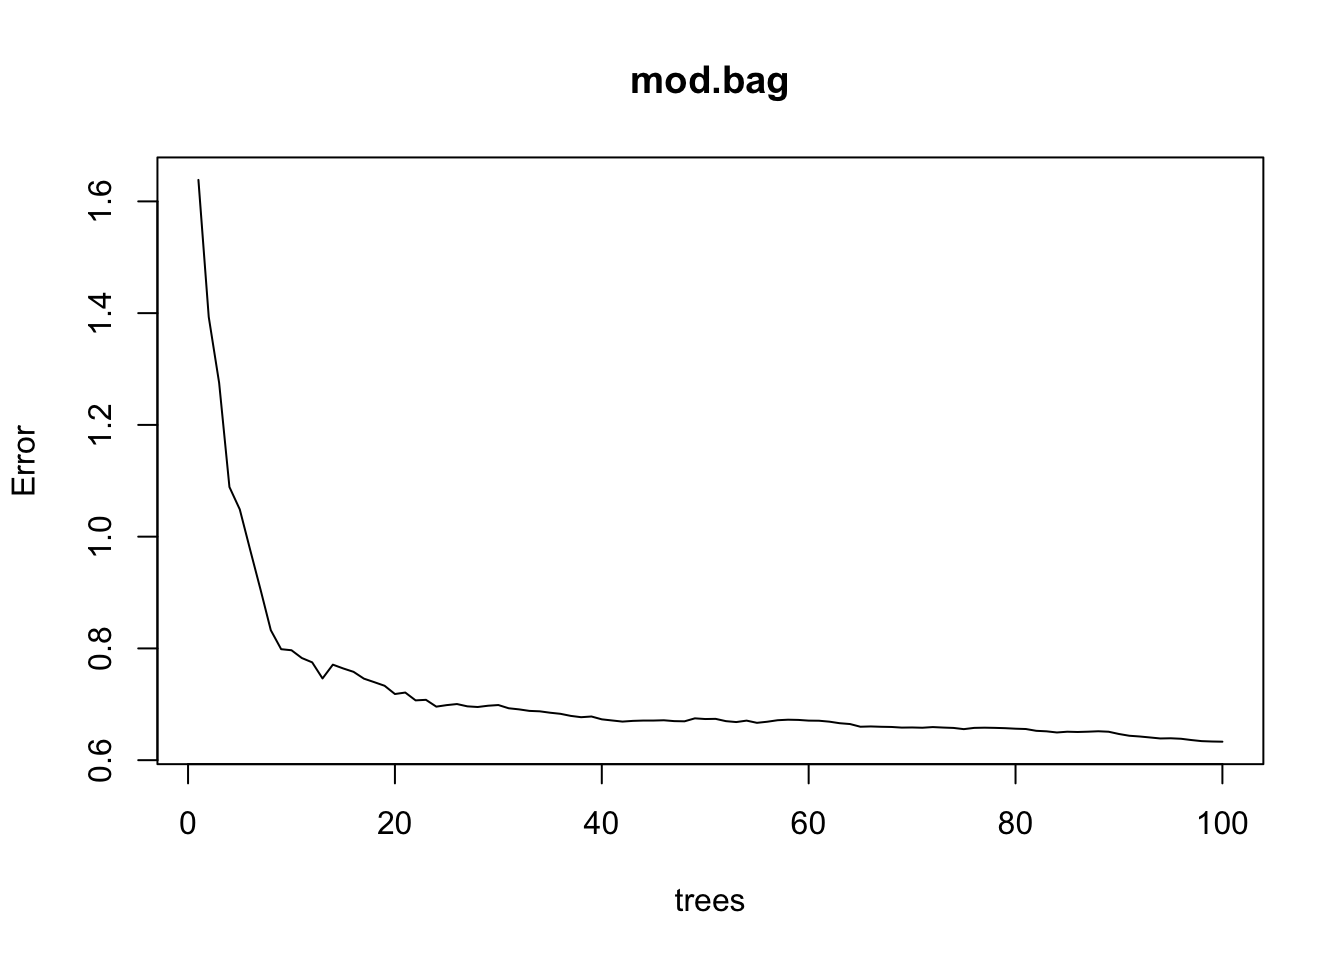
\includegraphics{introbagging_files/figure-latex/unnamed-chunk-17-1.pdf}
Bagging is nice because it is essentially impossible to overfit! The
more trees, the better. However, as this plot shows, there are
diminishing returns on the error rate decrease as the number of trees
increased. In any case, the only real limitation on the number of trees
is computing time (and your time).

Making predictions on the test data is easy.

\begin{Shaded}
\begin{Highlighting}[]
\NormalTok{preds.bag <-}\StringTok{ }\KeywordTok{predict}\NormalTok{(mod.bag,}
                     \DataTypeTok{newdata=}\NormalTok{test.df)}
\end{Highlighting}
\end{Shaded}

And computing the MSE on the test data.

\begin{Shaded}
\begin{Highlighting}[]
\NormalTok{(mse.bag <-}\StringTok{ }\KeywordTok{with}\NormalTok{(test.df,}\KeywordTok{mean}\NormalTok{((solubility }\OperatorTok{-}\StringTok{ }\NormalTok{preds.bag)}\OperatorTok{^}\DecValTok{2}\NormalTok{)))}
\end{Highlighting}
\end{Shaded}

\begin{verbatim}
## [1] 0.5242149
\end{verbatim}

Ok, this looks pretty good. We will, of course, compare this to the MSE
estimates from other prediction methods

\hypertarget{digging-deeper}{%
\subsubsection{Digging deeper}\label{digging-deeper}}

If you ask the model nicely, it will provide a great deal more
information. For example, for the test data, we can extract the error
rates from each of the numTree trees!

\begin{Shaded}
\begin{Highlighting}[]
\NormalTok{pred <-}\StringTok{ }\KeywordTok{predict}\NormalTok{(mod.bag,}
                \CommentTok{## Use test data}
                \DataTypeTok{newdata=}\NormalTok{test.df,}
                \CommentTok{## Keep predictions from all of the trees}
                \DataTypeTok{predict.all =} \OtherTok{TRUE}\NormalTok{) }
\end{Highlighting}
\end{Shaded}

Here are the final predictions for each observation.

\begin{Shaded}
\begin{Highlighting}[]
\NormalTok{predsBag <-}\StringTok{ }\NormalTok{pred}\OperatorTok{$}\NormalTok{aggregate}
\KeywordTok{length}\NormalTok{(predsBag)}
\end{Highlighting}
\end{Shaded}

\begin{verbatim}
## [1] 500
\end{verbatim}

For each observation, here are the predictions from each of the
individual trees! Note: One row for each observation, one column for
each tree

\begin{Shaded}
\begin{Highlighting}[]
\NormalTok{allPreds <-}\StringTok{ }\NormalTok{pred}\OperatorTok{$}\NormalTok{individual}
\KeywordTok{dim}\NormalTok{(allPreds)}
\end{Highlighting}
\end{Shaded}

\begin{verbatim}
## [1] 500 100
\end{verbatim}

For example, we could, if wanted, make a prediction from a single tree,
say the 10th one.

\begin{Shaded}
\begin{Highlighting}[]
\NormalTok{oneTree <-}\StringTok{ }\DecValTok{10}
\KeywordTok{with}\NormalTok{(test.df,}\KeywordTok{mean}\NormalTok{((allPreds[,oneTree]}\OperatorTok{-}\NormalTok{solubility)}\OperatorTok{^}\DecValTok{2}\NormalTok{))}
\end{Highlighting}
\end{Shaded}

\begin{verbatim}
## [1] 1.486667
\end{verbatim}

Not surprisingly, the prediction from a single tree isn't too
impressive.

Let's make predictions from each of the trees.

\begin{Shaded}
\begin{Highlighting}[]
\NormalTok{allErrs <-}\StringTok{ }\KeywordTok{map_dbl}\NormalTok{(}\DecValTok{1}\OperatorTok{:}\NormalTok{numTree,}
                   \ControlFlowTok{function}\NormalTok{(k) }\KeywordTok{with}\NormalTok{(test.df,}\KeywordTok{mean}\NormalTok{((allPreds[,k]}\OperatorTok{-}\NormalTok{solubility)}\OperatorTok{^}\DecValTok{2}\NormalTok{))   )}
\end{Highlighting}
\end{Shaded}

Let's look at a histogram of individual predictions

\begin{Shaded}
\begin{Highlighting}[]
\KeywordTok{ggplot}\NormalTok{()}\OperatorTok{+}
\StringTok{  }\KeywordTok{geom_histogram}\NormalTok{(}\KeywordTok{aes}\NormalTok{(allErrs),}\DataTypeTok{fill=}\StringTok{"blue"}\NormalTok{,}\DataTypeTok{color=}\StringTok{"white"}\NormalTok{,}\DataTypeTok{bins=}\DecValTok{20}\NormalTok{)}
\end{Highlighting}
\end{Shaded}

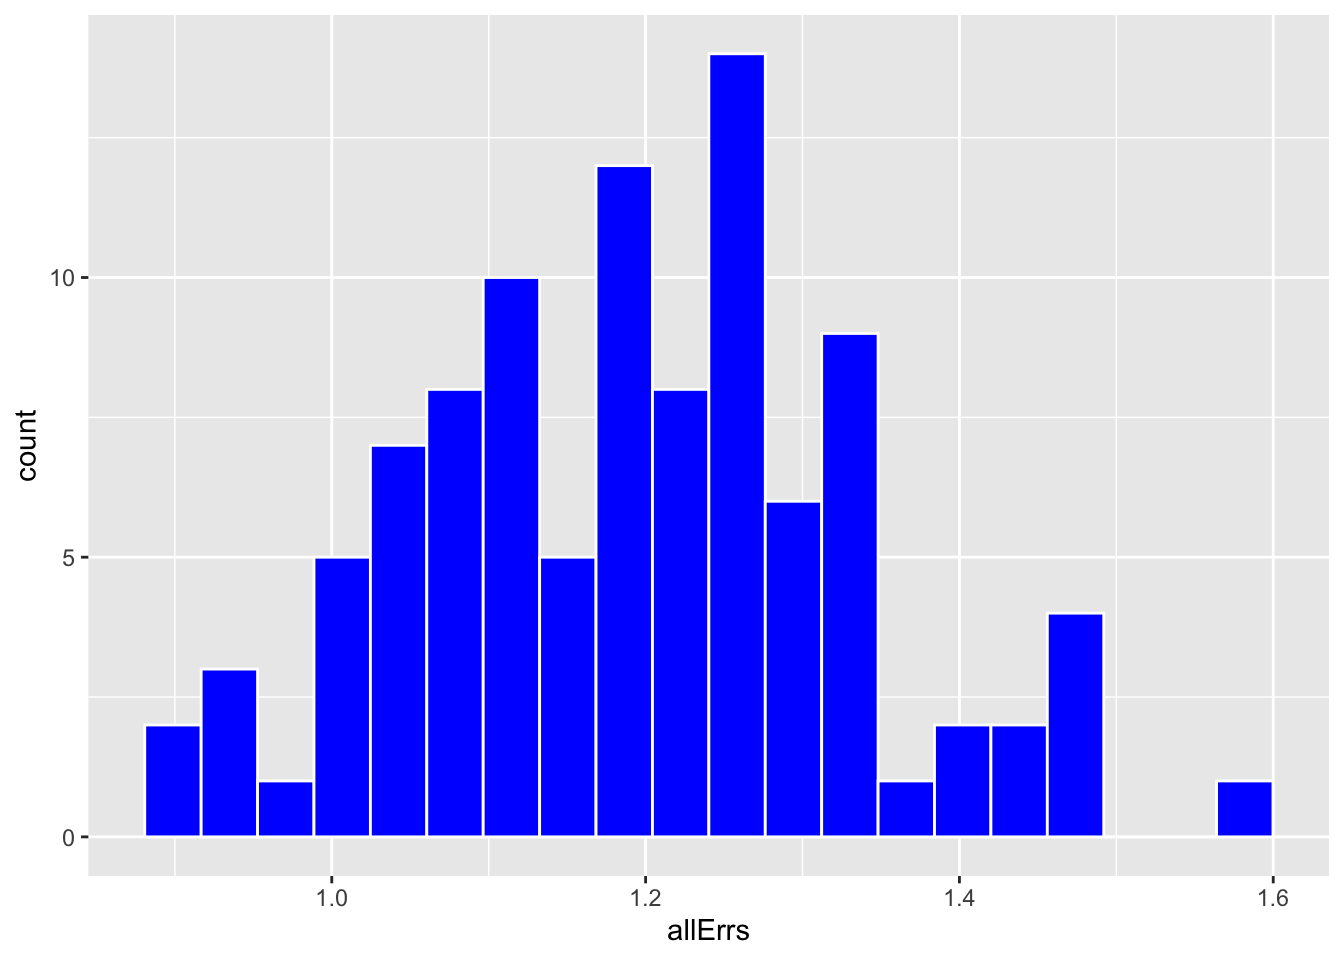
\includegraphics{introbagging_files/figure-latex/unnamed-chunk-25-1.pdf}
Not too good. The overall mean of the individual error rates isn't too
impressive: 1.2849646. Remember, the bagged tree has an overall MSE of
less than 0.5. At first it is odd to think that an individual tree has a
MSE near 1.0, but collectively they produce an error rate of 0.5.

\textbf{Wisdom of the Crowds}

We can easily retrieve the bagging estimate. Take the mean of each
row=observation. This is exactly the prediction of the randomForest.

\begin{Shaded}
\begin{Highlighting}[]
\NormalTok{meanPreds <-}\StringTok{ }\KeywordTok{apply}\NormalTok{(allPreds,}\DecValTok{1}\NormalTok{,mean)}
\KeywordTok{head}\NormalTok{(}\KeywordTok{cbind}\NormalTok{(meanPreds,predsBag))}
\end{Highlighting}
\end{Shaded}

\begin{verbatim}
##      meanPreds  predsBag
## 142  -2.693187 -2.693187
## 1050 -1.771842 -1.771842
## 670  -4.775325 -4.775325
## 90   -1.980210 -1.980210
## 712  -2.574527 -2.574527
## 893  -1.699427 -1.699427
\end{verbatim}

What if we only used the first 10 trees? How would this compare with
using all 100 trees?

\begin{Shaded}
\begin{Highlighting}[]
\NormalTok{subTrees <-}\StringTok{ }\DecValTok{10}
\NormalTok{somePreds <-}\StringTok{ }\NormalTok{allPreds[,}\DecValTok{1}\OperatorTok{:}\NormalTok{subTrees]}
\NormalTok{meanPreds <-}\StringTok{ }\KeywordTok{apply}\NormalTok{(somePreds,}\DecValTok{1}\NormalTok{,mean)}
\NormalTok{mse.bag10 <-}\StringTok{ }\KeywordTok{with}\NormalTok{(test.df,}\KeywordTok{mean}\NormalTok{((meanPreds}\OperatorTok{-}\NormalTok{solubility)}\OperatorTok{^}\DecValTok{2}\NormalTok{))}
\KeywordTok{c}\NormalTok{(mse.bag,mse.bag10)}
\end{Highlighting}
\end{Shaded}

\begin{verbatim}
## [1] 0.5242149 0.5738054
\end{verbatim}

As expected, the prediction isn't quite as good. In a similar way, we
could recreate plot(mod.bag) precisely. Try it.

\hypertarget{comparison-to-a-simple-linear-model}{%
\subsection{Comparison to a simple linear
model}\label{comparison-to-a-simple-linear-model}}

Now let's get a comparison to other methods. Start witha linear model
using all the predictors.

\begin{Shaded}
\begin{Highlighting}[]
\NormalTok{mod.lm <-}\StringTok{ }\KeywordTok{lm}\NormalTok{(solubility }\OperatorTok{~}\StringTok{ }\NormalTok{.,}
             \DataTypeTok{data=}\NormalTok{data.df)}
\NormalTok{preds.lm <-}\StringTok{ }\KeywordTok{predict}\NormalTok{(mod.lm,}\DataTypeTok{newdata=}\NormalTok{test.df)}
\end{Highlighting}
\end{Shaded}

\begin{verbatim}
## Warning in predict.lm(mod.lm, newdata = test.df): prediction from a rank-
## deficient fit may be misleading
\end{verbatim}

\begin{Shaded}
\begin{Highlighting}[]
\NormalTok{(mse.lm <-}\StringTok{ }\KeywordTok{with}\NormalTok{(test.df,}\KeywordTok{mean}\NormalTok{((solubility }\OperatorTok{-}\StringTok{ }\NormalTok{preds.lm)}\OperatorTok{^}\DecValTok{2}\NormalTok{)))}
\end{Highlighting}
\end{Shaded}

\begin{verbatim}
## [1] 0.7668777
\end{verbatim}

Note the warning coming out of the predict function. This indicates that
there is some serious correlations going on in the data set. One would
want to do some feature selection to clean it up.

Or, use penalized regression\ldots{}.. \#\# Ridge Regression

Now let's model with ridge regression. You could use lasso as well.

\begin{Shaded}
\begin{Highlighting}[]
\KeywordTok{suppressMessages}\NormalTok{(}\KeywordTok{library}\NormalTok{(glmnet))}
\end{Highlighting}
\end{Shaded}

Set up the data for glmnet.

\begin{Shaded}
\begin{Highlighting}[]
\NormalTok{data.x <-}\StringTok{ }\KeywordTok{data.matrix}\NormalTok{(data.df[,}\DecValTok{1}\OperatorTok{:}\NormalTok{numPred])}
\NormalTok{data.y <-}\StringTok{ }\KeywordTok{data.matrix}\NormalTok{(data.df[,numPred}\OperatorTok{+}\DecValTok{1}\NormalTok{])}
\end{Highlighting}
\end{Shaded}

Define a lambda grid and cross-validate.

\begin{Shaded}
\begin{Highlighting}[]
\NormalTok{lambda.grid <-}\StringTok{ }\DecValTok{10}\OperatorTok{^}\KeywordTok{seq}\NormalTok{(}\OperatorTok{-}\DecValTok{2}\NormalTok{,}\DecValTok{2}\NormalTok{,}\DataTypeTok{length=}\DecValTok{50}\NormalTok{)}
\NormalTok{mod.ridge.cv <-}\StringTok{ }\KeywordTok{cv.glmnet}\NormalTok{(data.x,data.y,}
                          \DataTypeTok{lambda=}\NormalTok{lambda.grid,}
                          \DataTypeTok{alpha=}\DecValTok{0}\NormalTok{)}
\KeywordTok{plot}\NormalTok{(mod.ridge.cv)}
\end{Highlighting}
\end{Shaded}

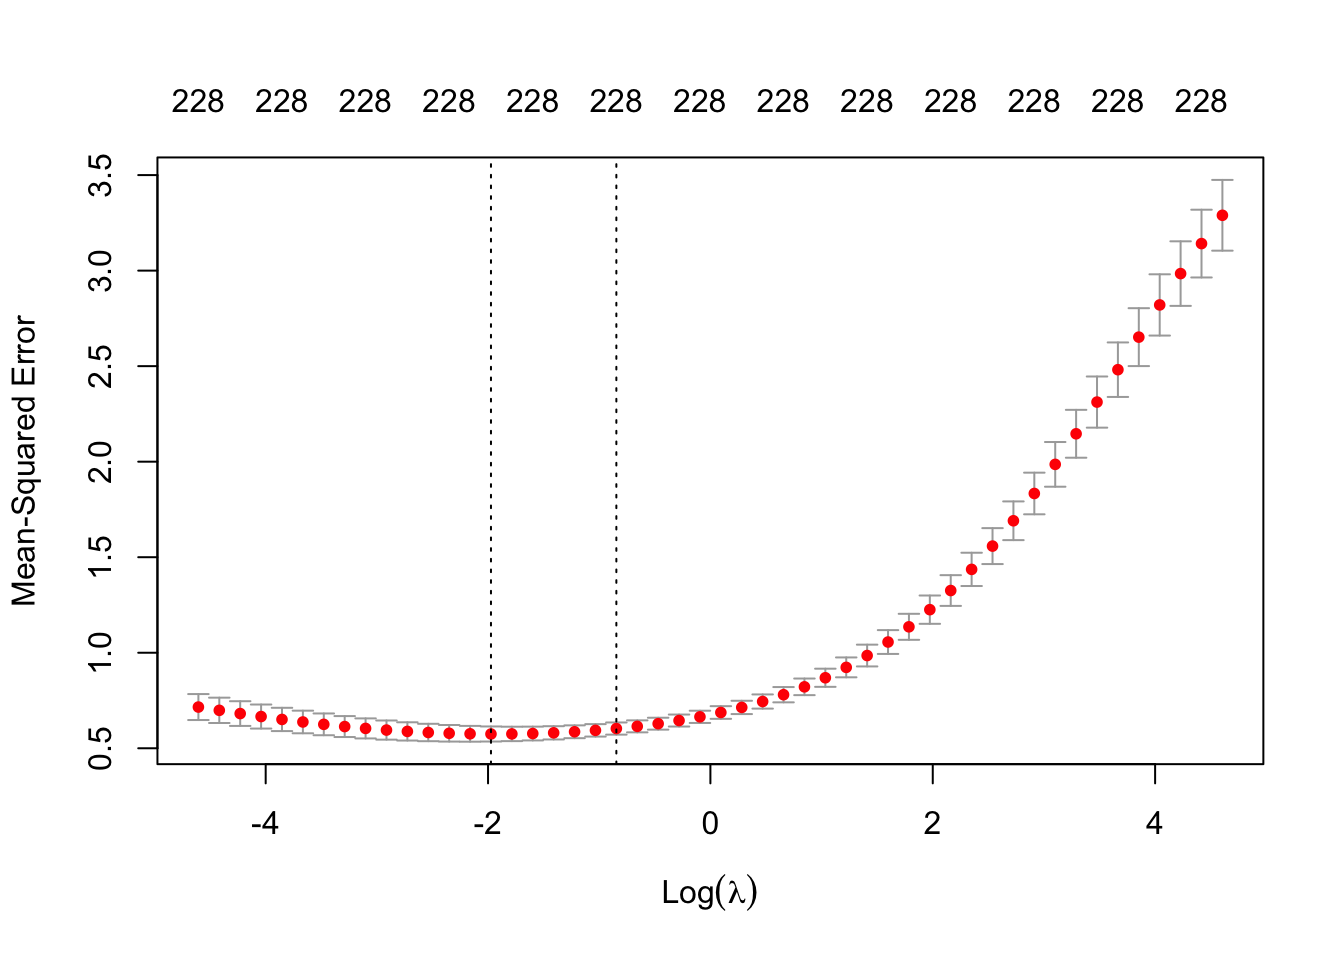
\includegraphics{introbagging_files/figure-latex/unnamed-chunk-31-1.pdf}

Kinda nice plot. There is a clear minimum indicating penalized
regression is warranted here. Use the One SE value and make predictions.

\begin{Shaded}
\begin{Highlighting}[]
\NormalTok{lambda.opt <-}\StringTok{ }\NormalTok{mod.ridge.cv}\OperatorTok{$}\NormalTok{lambda}\FloatTok{.1}\NormalTok{se}
\NormalTok{test.x <-}\StringTok{ }\KeywordTok{data.matrix}\NormalTok{(test.df[,}\DecValTok{1}\OperatorTok{:}\NormalTok{numPred])}
\NormalTok{test.y <-}\StringTok{ }\KeywordTok{data.matrix}\NormalTok{(test.df[,numPred}\OperatorTok{+}\DecValTok{1}\NormalTok{])}
\NormalTok{preds.ridge <-}\StringTok{ }\KeywordTok{predict}\NormalTok{(mod.ridge.cv,}\DataTypeTok{newx=}\NormalTok{test.x,}\DataTypeTok{s=}\NormalTok{lambda.opt)}
\NormalTok{(mse.ridge <-}\StringTok{ }\KeywordTok{with}\NormalTok{(test.df,}\KeywordTok{mean}\NormalTok{((solubility }\OperatorTok{-}\StringTok{ }\NormalTok{preds.ridge)}\OperatorTok{^}\DecValTok{2}\NormalTok{)))}
\end{Highlighting}
\end{Shaded}

\begin{verbatim}
## [1] 0.6131956
\end{verbatim}

Compare all the MSE values.

\begin{Shaded}
\begin{Highlighting}[]
\KeywordTok{c}\NormalTok{(mse.lm,mse.ridge,mse.bag)}
\end{Highlighting}
\end{Shaded}

\begin{verbatim}
## [1] 0.7668777 0.6131956 0.5242149
\end{verbatim}

So far, Bagging is winning.

\hypertarget{random-forests}{%
\section{Random Forests}\label{random-forests}}

Random forests introduce a twist to the bagging process. Instead of
using all the predictors at each branch, only use a random subset of a
particular size.

Why? Using all the predictors favors the ``heavy hitters'' each time.
Even with bootstrapping, the same small set of predictors tend to
dominate the branching decisions, at least early on when a lot of the
MSE is accounted for. This means the bootstrapped trees are not entirely
independent of each other.

By limiting to a fraction of the predictors each time, more predictors
get a chance to play a role in the tree construction, especially at the
early stages. This leads to trees which are much more independent of
each other and hence more randomization of the predictions.

The number of predictors at each branch is controled by the randomForest
parameter ``mtry''. There is no ``best'' value for mtry, but it has been
found that if numPred is the total number of predictors, numPred/3 or
sqrt(numPred) work well.

Let's build a random forest with numPred/3 predictors at each step.

\begin{Shaded}
\begin{Highlighting}[]
\NormalTok{mod.rf <-}\StringTok{ }\KeywordTok{randomForest}\NormalTok{(solubility }\OperatorTok{~}\StringTok{ }\NormalTok{.,}
                       \DataTypeTok{data=}\NormalTok{data.df,}
                       \DataTypeTok{ntree=}\NormalTok{numTree,}
                       \CommentTok{## Limit to 1/3 of predictors at each branch}
                       \DataTypeTok{mtry=}\NormalTok{(numPred)}\OperatorTok{/}\DecValTok{3}\NormalTok{)}
\NormalTok{mod.rf}
\end{Highlighting}
\end{Shaded}

\begin{verbatim}
## 
## Call:
##  randomForest(formula = solubility ~ ., data = data.df, ntree = numTree,      mtry = (numPred)/3) 
##                Type of random forest: regression
##                      Number of trees: 100
## No. of variables tried at each split: 76
## 
##           Mean of squared residuals: 0.5756111
##                     % Var explained: 87.32
\end{verbatim}

Again, the ``Mean of squared residuals'' is the OOB estimate.

The plot is similar.

\begin{Shaded}
\begin{Highlighting}[]
\KeywordTok{plot}\NormalTok{(mod.rf)}
\end{Highlighting}
\end{Shaded}

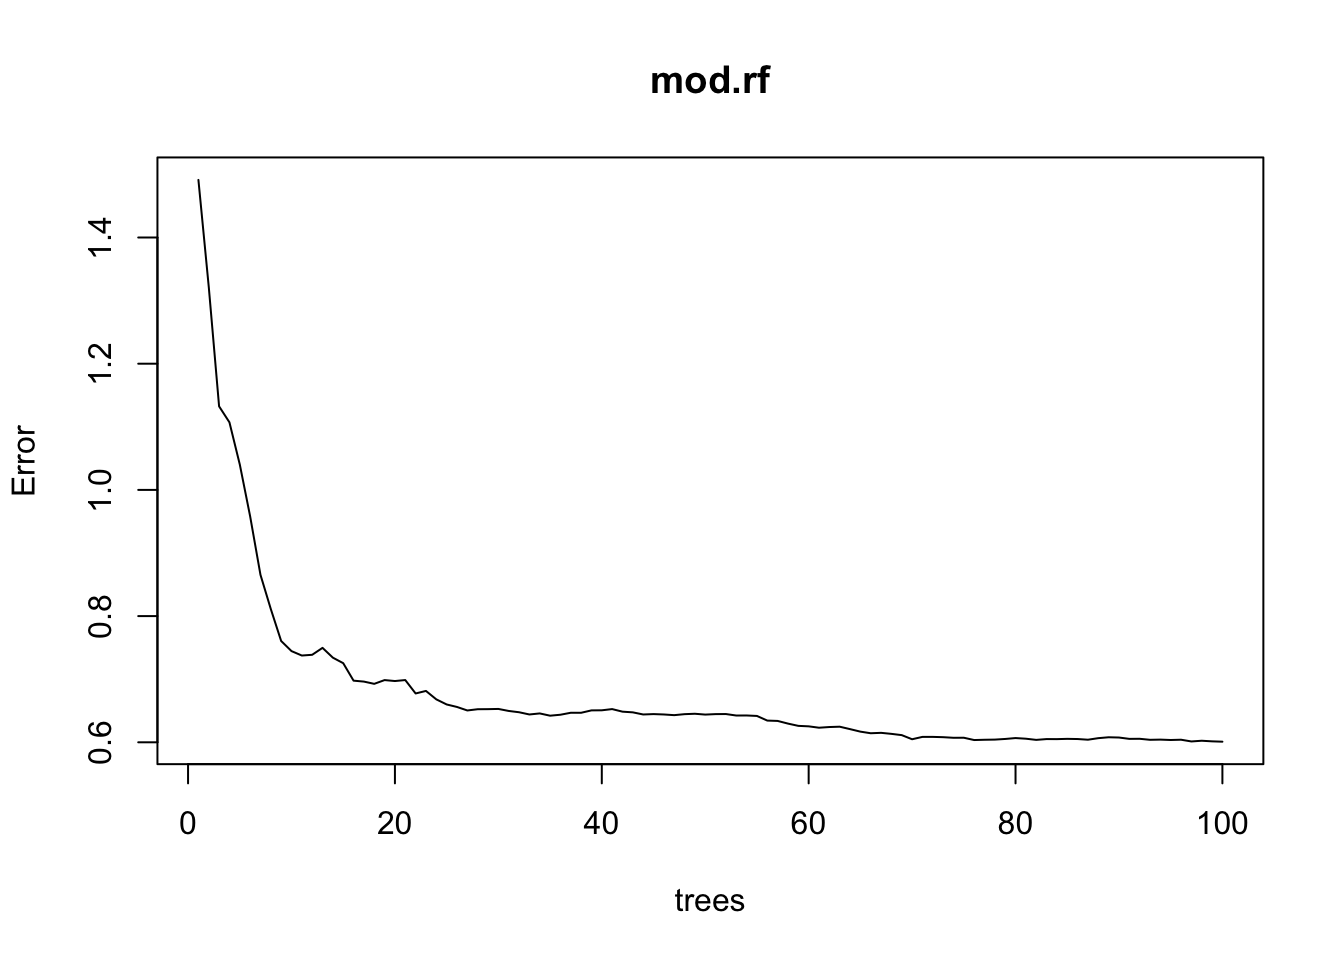
\includegraphics{introbagging_files/figure-latex/unnamed-chunk-35-1.pdf}

As before, we can make the predictions for each observation and compare
with the other mse values.

\begin{Shaded}
\begin{Highlighting}[]
\NormalTok{preds.rf <-}\StringTok{ }\KeywordTok{predict}\NormalTok{(mod.rf,}\DataTypeTok{newdata=}\NormalTok{test.df)}
\NormalTok{(mse.rf <-}\StringTok{ }\KeywordTok{with}\NormalTok{(test.df,}\KeywordTok{mean}\NormalTok{((solubility }\OperatorTok{-}\StringTok{ }\NormalTok{preds.rf)}\OperatorTok{^}\DecValTok{2}\NormalTok{)))}
\end{Highlighting}
\end{Shaded}

\begin{verbatim}
## [1] 0.4985529
\end{verbatim}

How do the four methods stack up?

\begin{Shaded}
\begin{Highlighting}[]
\KeywordTok{c}\NormalTok{(mse.lm,mse.ridge,mse.bag,mse.rf)}
\end{Highlighting}
\end{Shaded}

\begin{verbatim}
## [1] 0.7668777 0.6131956 0.5242149 0.4985529
\end{verbatim}

It looks as if the bagging models outperform regression (simple or
penalized) in this case.

\hypertarget{assignment-2}{%
\subsection{Assignment}\label{assignment-2}}

For the solubility data, compute the analog of Figure 17.2 of Compute
Age Statistical Inference.

\url{https://web.stanford.edu/~hastie/CASI_files/PDF/casi.pdf}

Note: Replace Lasso (interactions) with Ridge Regression.

Do you reach the same conclusion, namely that bagging/random forests
outperform the other models? \# Predictor Importance As we build
different bootstrapped versions of the data and hence different trees,
the predictors get used in different ways. This is especially true of a
random forest when mtry is something like numPred/3.

We can measure the impact of a variable by keeping track of how much the
MSE (or error rate, or binomial deviance, etc) changes each time that
predictor is used. The total of all these changes in guage of the
predictors ``Importance''.

Importance variables are very helpful when it comes to trying to explain
the results of a random forest model. We can't talk about 1000 or so
trees, but we can talk about how various predictors impact the final
predictions.

Fortunately, the R randomForest function keeps track of this
information.

\begin{Shaded}
\begin{Highlighting}[]
\NormalTok{mod.rf <-}\StringTok{ }\KeywordTok{randomForest}\NormalTok{(solubility }\OperatorTok{~}\StringTok{ }\NormalTok{.,}
                       \DataTypeTok{data=}\NormalTok{data.df,}
                       \DataTypeTok{ntree=}\NormalTok{numTree,}
                       \CommentTok{## Limit to 1/3 of predictors at each branch}
                       \DataTypeTok{mtry=}\NormalTok{(numPred)}\OperatorTok{/}\DecValTok{3}\NormalTok{,}
                       \CommentTok{## Include this flag}
                       \DataTypeTok{importance=}\OtherTok{TRUE}\NormalTok{)}
\end{Highlighting}
\end{Shaded}

Here's a bare-bones look at importance.

\begin{Shaded}
\begin{Highlighting}[]
\KeywordTok{varImpPlot}\NormalTok{(mod.rf)}
\end{Highlighting}
\end{Shaded}

\includegraphics{introbagging_files/figure-latex/unnamed-chunk-39-1.pdf}
Importance can be viewed from both a MSE reduction perspective and Node
Purity perspective. We can that the predictor ``MolWeight'' plays the
large role.

The plot looks much better zoomed. \#\# Improved Importance Plot This
plot is not much too look at. We can fix this up pretty easily and make
it more presentable.

\begin{Shaded}
\begin{Highlighting}[]
\KeywordTok{head}\NormalTok{(mod.rf}\OperatorTok{$}\NormalTok{importance)}
\end{Highlighting}
\end{Shaded}

\begin{verbatim}
##           %IncMSE IncNodePurity
## FP001 0.005651421     0.9306213
## FP002 0.016411124     1.4518659
## FP003 0.002771210     2.1738827
## FP004 0.026507844     7.2299262
## FP005 0.002547468     0.6271920
## FP006 0.009107189     2.1601412
\end{verbatim}

\begin{Shaded}
\begin{Highlighting}[]
\CommentTok{## grab the importance values}
\NormalTok{importVals <-mod.rf}\OperatorTok{$}\NormalTok{importance }\CommentTok{# importance(mod.rf)}
\CommentTok{## Just use  MSE}
\NormalTok{importVals <-}\StringTok{ }\NormalTok{importVals[,}\DecValTok{1}\NormalTok{]}
\CommentTok{## and the names}
\NormalTok{varNames <-}\StringTok{ }\KeywordTok{row.names}\NormalTok{(mod.rf}\OperatorTok{$}\NormalTok{importance)}
\end{Highlighting}
\end{Shaded}

Pack all this into a nice data frame.

\begin{Shaded}
\begin{Highlighting}[]
\NormalTok{importanceRF.df <-}\StringTok{ }\KeywordTok{data.frame}\NormalTok{(}\DataTypeTok{importance=}\NormalTok{importVals,}
                              \DataTypeTok{var=}\NormalTok{varNames)}\OperatorTok
\StringTok{  }\KeywordTok{arrange}\NormalTok{(}\KeywordTok{desc}\NormalTok{(importance))}
\end{Highlighting}
\end{Shaded}

Fix the order of the var factor (otherwise R will want to put them in
alphabetical order).

\begin{Shaded}
\begin{Highlighting}[]
\NormalTok{varNames <-}\StringTok{ }\NormalTok{importanceRF.df}\OperatorTok{$}\NormalTok{var}
\NormalTok{importanceRF.df <-}\StringTok{ }\NormalTok{importanceRF.df}\OperatorTok
\StringTok{  }\KeywordTok{mutate}\NormalTok{(}\DataTypeTok{var=}\KeywordTok{factor}\NormalTok{(var,}\DataTypeTok{levels=}\KeywordTok{rev}\NormalTok{(varNames)))}
\end{Highlighting}
\end{Shaded}

And the Importance Plot\ldots{}

\begin{Shaded}
\begin{Highlighting}[]
\CommentTok{##only show the top 25}
\NormalTok{rf.gg <-}\StringTok{ }\NormalTok{importanceRF.df[}\DecValTok{1}\OperatorTok{:}\DecValTok{25}\NormalTok{,] }\OperatorTok
\StringTok{  }\KeywordTok{ggplot}\NormalTok{()}\OperatorTok{+}
\StringTok{  }\KeywordTok{geom_bar}\NormalTok{(}\KeywordTok{aes}\NormalTok{(var,importance),}\DataTypeTok{stat=}\StringTok{"identity"}\NormalTok{,}\DataTypeTok{fill=}\StringTok{"red"}\NormalTok{)}\OperatorTok{+}
\StringTok{  }\KeywordTok{coord_flip}\NormalTok{()}\OperatorTok{+}
\StringTok{  }\KeywordTok{labs}\NormalTok{(}\DataTypeTok{title=}\StringTok{"Importance of Predictors"}\NormalTok{,}
       \DataTypeTok{subtitle=}\StringTok{"Random Forest"}\NormalTok{,}
       \DataTypeTok{x=}\StringTok{""}\NormalTok{,}
       \DataTypeTok{y=}\StringTok{""}\NormalTok{)}
\NormalTok{rf.gg}
\end{Highlighting}
\end{Shaded}

\includegraphics{introbagging_files/figure-latex/importPlot-1.pdf} It's
interesting to compare the importance plot to to that of a bagged model.

\begin{Shaded}
\begin{Highlighting}[]
\CommentTok{## Random Forests can supply imformation about the impact of each predictor}
\NormalTok{mod.bag <-}\StringTok{ }\KeywordTok{randomForest}\NormalTok{(solubility }\OperatorTok{~}\StringTok{ }\NormalTok{.,}
                        \DataTypeTok{data=}\NormalTok{data.df,}
                        \DataTypeTok{ntree=}\NormalTok{numTree,}
                        \CommentTok{## BAGGING }
                        \DataTypeTok{mtry=}\NormalTok{(numPred),}
                        \CommentTok{## Include this flag}
                        \DataTypeTok{importance=}\OtherTok{TRUE}\NormalTok{)}
\CommentTok{#### grab the importance values}
\NormalTok{importVals <-mod.bag}\OperatorTok{$}\NormalTok{importance }\CommentTok{# importance(mod.rf)}
\CommentTok{## Just use  MSE}
\NormalTok{importVals <-}\StringTok{ }\NormalTok{importVals[,}\DecValTok{1}\NormalTok{]}
\CommentTok{## and the names}
\NormalTok{varNames <-}\StringTok{ }\KeywordTok{row.names}\NormalTok{(mod.rf}\OperatorTok{$}\NormalTok{importance)}
\NormalTok{importanceBag.df <-}\StringTok{ }\KeywordTok{data.frame}\NormalTok{(}\DataTypeTok{importance=}\NormalTok{importVals,}
                               \DataTypeTok{var=}\NormalTok{varNames)}\OperatorTok
\StringTok{  }\KeywordTok{arrange}\NormalTok{(}\KeywordTok{desc}\NormalTok{(importance))}
\CommentTok{##}
\NormalTok{varNames <-}\StringTok{ }\NormalTok{importanceBag.df}\OperatorTok{$}\NormalTok{var}
\NormalTok{importanceBag.df <-importanceBag.df}\OperatorTok
\StringTok{  }\KeywordTok{mutate}\NormalTok{(}\DataTypeTok{var=}\KeywordTok{factor}\NormalTok{(var,}\DataTypeTok{levels=}\KeywordTok{rev}\NormalTok{(varNames)))}

\CommentTok{##only show the top 25}
\NormalTok{bag.gg <-}\StringTok{ }\NormalTok{importanceBag.df[}\DecValTok{1}\OperatorTok{:}\DecValTok{25}\NormalTok{,] }\OperatorTok
\StringTok{  }\KeywordTok{ggplot}\NormalTok{()}\OperatorTok{+}
\StringTok{  }\KeywordTok{geom_bar}\NormalTok{(}\KeywordTok{aes}\NormalTok{(var,importance),}\DataTypeTok{stat=}\StringTok{"identity"}\NormalTok{,}\DataTypeTok{fill=}\StringTok{"red"}\NormalTok{)}\OperatorTok{+}
\StringTok{  }\KeywordTok{coord_flip}\NormalTok{()}\OperatorTok{+}
\StringTok{  }\KeywordTok{labs}\NormalTok{(}\DataTypeTok{title=}\StringTok{"Importance of Predictors"}\NormalTok{,}
       \DataTypeTok{subtitle=}\StringTok{"Bagging"}\NormalTok{,}
       \DataTypeTok{x=}\StringTok{""}\NormalTok{,}
       \DataTypeTok{y=}\StringTok{""}\NormalTok{)}
\NormalTok{bag.gg}
\end{Highlighting}
\end{Shaded}

\includegraphics{introbagging_files/figure-latex/unnamed-chunk-43-1.pdf}

The two importance plots are similar, but there are some differences in
the order of importance.

\begin{Shaded}
\begin{Highlighting}[]
\KeywordTok{library}\NormalTok{(gridExtra)}
\end{Highlighting}
\end{Shaded}

\begin{verbatim}
## 
## Attaching package: 'gridExtra'
\end{verbatim}

\begin{verbatim}
## The following object is masked from 'package:randomForest':
## 
##     combine
\end{verbatim}

\begin{verbatim}
## The following object is masked from 'package:dplyr':
## 
##     combine
\end{verbatim}

\begin{Shaded}
\begin{Highlighting}[]
\KeywordTok{grid.arrange}\NormalTok{(bag.gg,rf.gg,}\DataTypeTok{nrow=}\DecValTok{1}\NormalTok{)}
\end{Highlighting}
\end{Shaded}

\includegraphics{introbagging_files/figure-latex/unnamed-chunk-44-1.pdf}

\hypertarget{summary}{%
\section{Summary}\label{summary}}

Bagging, and Random Forests, in particular have proven to be very robust
tools for prediction. In almost all cases, Random Forests are
competitive with regression methods. Moreover, in many cases, Random
Forests are demonstratively better methods. With Importance Plots, they
also have a nice descriptive feature that makes them useful even for
decriptive analysis.

\hypertarget{assignment-1-1}{%
\subsection{Assignment 1}\label{assignment-1-1}}

Modify our bootstrapped method above so that it computes a class
prediction for each observation. Make sure that your results agree (up
to randomness) with the randomForest function

Plan: Create a matrix with one row for each observation and one column
for each tree (bootstrap). Each time through, put the OOB predictions
into their rows of the matrix (the column is the current boot strap
index). Careful: the predictions from the tree are usually given values
1,2, instead of ``A'', ``B''.

When done, do a majority vote across each row. In each row, only about
1/3 of the values will be filled in. You have to ignore the NAs.

\begin{Shaded}
\begin{Highlighting}[]
\NormalTok{N <-}\StringTok{ }\KeywordTok{nrow}\NormalTok{(classData.df)}
\NormalTok{n <-}\StringTok{ }\DecValTok{200}
\NormalTok{build <-}\StringTok{ }\KeywordTok{sample}\NormalTok{(}\DecValTok{1}\OperatorTok{:}\NormalTok{N,n,}\DataTypeTok{rep=}\NormalTok{F) }
\NormalTok{data.df <-}\StringTok{ }\NormalTok{classData.df[build,]}
\NormalTok{numTree <-}\StringTok{ }\DecValTok{100}
\NormalTok{numPred <-}\StringTok{ }\DecValTok{2}
\NormalTok{mod.bag <-}\StringTok{ }\KeywordTok{randomForest}\NormalTok{(class }\OperatorTok{~}\StringTok{ }\NormalTok{x }\OperatorTok{+}\StringTok{ }\NormalTok{y,}
                        \DataTypeTok{data=}\NormalTok{data.df, }
                        \DataTypeTok{ntree=}\NormalTok{numTree, }
                        \DataTypeTok{mtry=}\NormalTok{numPred)}
\NormalTok{mod.bag}\OperatorTok{$}\NormalTok{confusion}
\end{Highlighting}
\end{Shaded}

\begin{verbatim}
##    A  B class.error
## A 82 20   0.1960784
## B 21 77   0.2142857
\end{verbatim}

\begin{Shaded}
\begin{Highlighting}[]
\KeywordTok{mean}\NormalTok{(mod.bag}\OperatorTok{$}\NormalTok{err.rate)}
\end{Highlighting}
\end{Shaded}

\begin{verbatim}
## [1] 0.2203914
\end{verbatim}

\begin{Shaded}
\begin{Highlighting}[]
\NormalTok{numBoots <-}\StringTok{ }\DecValTok{100}
\NormalTok{bootedTrees <-}\StringTok{ }\KeywordTok{list}\NormalTok{()}
\NormalTok{oobPreds <-}\StringTok{ }\KeywordTok{matrix}\NormalTok{(}\DataTypeTok{nrow=}\KeywordTok{nrow}\NormalTok{(data.df),}\DataTypeTok{ncol=}\NormalTok{numBoots) }
\ControlFlowTok{for}\NormalTok{(k }\ControlFlowTok{in} \DecValTok{1}\OperatorTok{:}\NormalTok{numBoots)\{}
\NormalTok{  boots <-}\StringTok{ }\KeywordTok{sample}\NormalTok{(}\DecValTok{1}\OperatorTok{:}\NormalTok{n,n,}\DataTypeTok{rep=}\NormalTok{T) }
\NormalTok{  boot.df <-}\StringTok{ }\NormalTok{data.df[boots,]}
\NormalTok{  oobs <-}\StringTok{ }\KeywordTok{setdiff}\NormalTok{(}\DecValTok{1}\OperatorTok{:}\NormalTok{n,boots) }
\NormalTok{  oob.df <-}\StringTok{ }\NormalTok{data.df[oobs,] }
\NormalTok{  bootedTree <-}\StringTok{ }\KeywordTok{tree}\NormalTok{(class }\OperatorTok{~}\StringTok{ }\NormalTok{x}\OperatorTok{+}\NormalTok{y,}
                     \DataTypeTok{data =}\NormalTok{ boot.df,}
                     \DataTypeTok{control =} \KeywordTok{tree.control}\NormalTok{(}\KeywordTok{nrow}\NormalTok{(boot.df),}\DataTypeTok{mindev =} \DecValTok{0}\NormalTok{,}\DecValTok{001}\NormalTok{,}\DataTypeTok{minsize =} \DecValTok{2}\NormalTok{))}
\NormalTok{  preds <-}\StringTok{ }\KeywordTok{predict}\NormalTok{(bootedTree,}
                   \DataTypeTok{newdata =}\NormalTok{ oob.df,}
                   \DataTypeTok{type =} \StringTok{"class"}\NormalTok{)}
\NormalTok{  oobPreds[oobs,k] <-}\StringTok{ }\NormalTok{preds}
\NormalTok{\}}
\NormalTok{oobA <-}\StringTok{ }\KeywordTok{apply}\NormalTok{(oobPreds,}\DecValTok{1}\NormalTok{,}\ControlFlowTok{function}\NormalTok{(vals) }\KeywordTok{sum}\NormalTok{(vals}\OperatorTok{==}\StringTok{"1"}\NormalTok{,}\DataTypeTok{na.rm=}\NormalTok{T)) }
\NormalTok{oobB <-}\StringTok{ }\KeywordTok{apply}\NormalTok{(oobPreds,}\DecValTok{1}\NormalTok{,}\ControlFlowTok{function}\NormalTok{(vals) }\KeywordTok{sum}\NormalTok{(vals}\OperatorTok{==}\StringTok{"2"}\NormalTok{,}\DataTypeTok{na.rm=}\NormalTok{T)) }
\NormalTok{preds <-}\StringTok{ }\KeywordTok{ifelse}\NormalTok{(oobA }\OperatorTok{>=}\StringTok{ }\NormalTok{oobB,}\StringTok{"A"}\NormalTok{,}\StringTok{"B"}\NormalTok{) }
\KeywordTok{with}\NormalTok{(data.df,}\KeywordTok{table}\NormalTok{(class,preds))}
\end{Highlighting}
\end{Shaded}

\begin{verbatim}
##      preds
## class  A  B
##     A 82 20
##     B 22 76
\end{verbatim}

\begin{Shaded}
\begin{Highlighting}[]
\KeywordTok{with}\NormalTok{(data.df,}\KeywordTok{mean}\NormalTok{(class }\OperatorTok{!=}\StringTok{ }\NormalTok{preds))}
\end{Highlighting}
\end{Shaded}

\begin{verbatim}
## [1] 0.21
\end{verbatim}

They share pretty similar error rate.

\hypertarget{assignment-2-1}{%
\subsection{Assignment 2}\label{assignment-2-1}}

Replicate the results computed in mod.bag using a modification (to
perform regression instead of classification) of the bootstrapping done
above. For each bootstrapped tree, keep track of the oob predictions.

When done, use these to make a prediction for each observation and then
use these to estimate the MSE.

Compare you bootstrapped prediction and oob MSE with the results from
mod.bag. They should be very similar.

\begin{Shaded}
\begin{Highlighting}[]
\NormalTok{N <-}\StringTok{ }\KeywordTok{nrow}\NormalTok{(solubil.df)}
\NormalTok{n <-}\StringTok{ }\DecValTok{200}
\NormalTok{build <-}\StringTok{ }\KeywordTok{sample}\NormalTok{(}\DecValTok{1}\OperatorTok{:}\NormalTok{N,n,}\DataTypeTok{rep=}\NormalTok{F) }
\NormalTok{data.df <-}\StringTok{ }\NormalTok{solubil.df[build,]}
\NormalTok{numTree <-}\StringTok{ }\DecValTok{100}
\NormalTok{mod.bag <-}\StringTok{ }\KeywordTok{randomForest}\NormalTok{(solubility }\OperatorTok{~}\NormalTok{.,}
                        \DataTypeTok{data=}\NormalTok{data.df, }
                        \DataTypeTok{ntree=}\NormalTok{numTree, }
                        \DataTypeTok{mtry=}\NormalTok{numPred)}
\KeywordTok{mean}\NormalTok{(mod.bag}\OperatorTok{$}\NormalTok{mse)}
\end{Highlighting}
\end{Shaded}

\begin{verbatim}
## [1] 1.591393
\end{verbatim}

\begin{Shaded}
\begin{Highlighting}[]
\NormalTok{numBoots <-}\StringTok{ }\DecValTok{100}
\NormalTok{bootedTrees <-}\StringTok{ }\KeywordTok{list}\NormalTok{()}
\NormalTok{oobPreds <-}\StringTok{ }\KeywordTok{matrix}\NormalTok{(}\DataTypeTok{nrow=}\KeywordTok{nrow}\NormalTok{(data.df),}\DataTypeTok{ncol=}\NormalTok{numBoots) }
\ControlFlowTok{for}\NormalTok{(k }\ControlFlowTok{in} \DecValTok{1}\OperatorTok{:}\NormalTok{numBoots)\{}
\NormalTok{  boots <-}\StringTok{ }\KeywordTok{sample}\NormalTok{(}\DecValTok{1}\OperatorTok{:}\NormalTok{n,n,}\DataTypeTok{rep=}\NormalTok{T) }
\NormalTok{  boot.df <-}\StringTok{ }\NormalTok{data.df[boots,]}
\NormalTok{  oobs <-}\StringTok{ }\KeywordTok{setdiff}\NormalTok{(}\DecValTok{1}\OperatorTok{:}\NormalTok{n,boots) }
\NormalTok{  oob.df <-}\StringTok{ }\NormalTok{data.df[oobs,] }
\NormalTok{  bootedTree <-}\StringTok{ }\KeywordTok{tree}\NormalTok{(solubility }\OperatorTok{~}\NormalTok{.,}
                     \DataTypeTok{data =}\NormalTok{ boot.df,}
                     \DataTypeTok{control =} \KeywordTok{tree.control}\NormalTok{(}\KeywordTok{nrow}\NormalTok{(boot.df),}
                                            \DataTypeTok{mindev =} \DecValTok{0}\NormalTok{,}\DecValTok{001}\NormalTok{,}
                                            \DataTypeTok{minsize =} \DecValTok{2}\NormalTok{))}
\NormalTok{  preds <-}\StringTok{ }\KeywordTok{predict}\NormalTok{(bootedTree,}
                   \DataTypeTok{newdata =}\NormalTok{ oob.df,)}
\NormalTok{  oobPreds[oobs,k] <-}\StringTok{ }\NormalTok{preds}
\NormalTok{\}}

\NormalTok{meanPreds <-}\StringTok{ }\KeywordTok{apply}\NormalTok{(oobPreds,}\DecValTok{1}\NormalTok{,}\ControlFlowTok{function}\NormalTok{(vals) }\KeywordTok{mean}\NormalTok{(vals,}\DataTypeTok{na.rm=}\NormalTok{T)) }
\NormalTok{mseBoots <-}\StringTok{ }\KeywordTok{with}\NormalTok{(data.df, }\KeywordTok{mean}\NormalTok{((meanPreds}\OperatorTok{-}\NormalTok{solubility)}\OperatorTok{^}\DecValTok{2}\NormalTok{))}
\KeywordTok{c}\NormalTok{(mseBoots)}
\end{Highlighting}
\end{Shaded}

\begin{verbatim}
## [1] 0.605984
\end{verbatim}

\end{document}
